


%\subsection{Aprendizaje automático}
\begin{frame}{\citetitle{MarcoNuno_CongArbIng_2015_02_00} \footnotemark (1) }
\begin{columns}
\begin{column}{0.4\textwidth}
		Componentes:
		\begin{itemize}
		\item Captura de datos del acelerómetro del teléfono
		\item Procesar los datos empleando algoritmos de ML previamente entrenados, para determinar el tipo de actividad llevada a cabo por el usuario
		\end{itemize}
\end{column}
\begin{column}{0.6\textwidth}  
    \begin{center}
     %%%%% this is a minipage, so \textwidth is already adjusted to the size of the column
     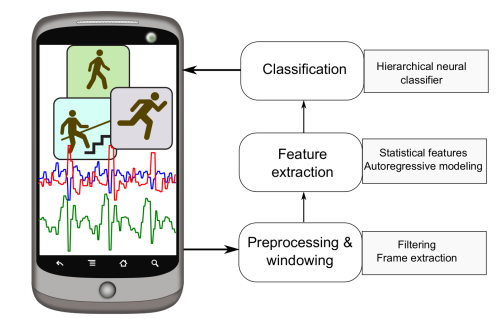
\includegraphics[width=0.8\textwidth]{Figs/DeteccionActividad1}
     \end{center}
\end{column}
\end{columns}
\footnotetext[1]{\fullcite{MarcoNuno_CongArbIng_2015_02_00}}
\setcounter{footnote}{0}
\end{frame}


\begin{frame}{\citetitle{MarcoNuno_CongArbIng_2015_02_00} \footnotemark (2) }
\begin{columns}
\begin{column}{0.40\textwidth}
		Componentes:
		\begin{itemize}
		\item Se empleo una red neuronal jerárquica
		\item Se midió el desempeño de la bateria y los tiempos de los principales pasos
		\end{itemize}
\begin{center}
     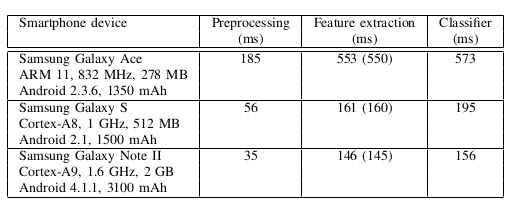
\includegraphics[width=0.7\textwidth]{Figs/DeteccionActividad3}
     
     \end{center}
\end{column}
\begin{column}{0.29\textwidth}  
    \begin{center}
     %%%%% this is a minipage, so \textwidth is already adjusted to the size of the column
     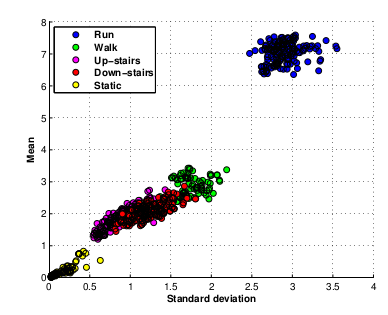
\includegraphics[width=0.97\textwidth]{Figs/DeteccionActividad2}
	%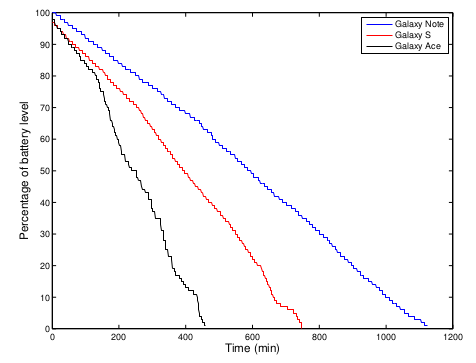
\includegraphics[width=0.7\textwidth]{Figs/DeteccionActividad4}

     \end{center}
\end{column}
\begin{column}{0.29\textwidth}  
    \begin{center}
     %%%%% this is a minipage, so \textwidth is already adjusted to the size of the column
     %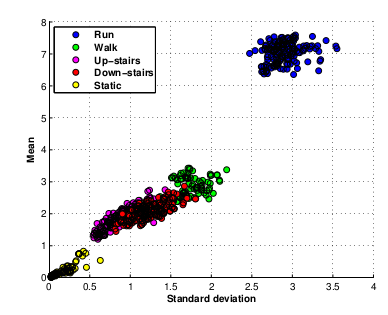
\includegraphics[width=0.7\textwidth]{Figs/DeteccionActividad2}
	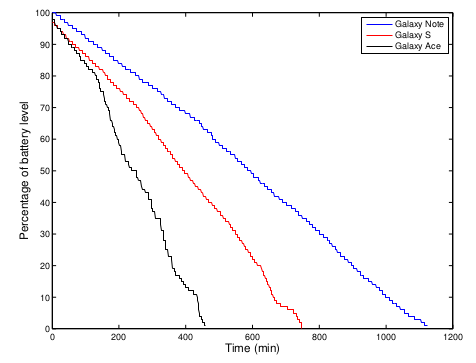
\includegraphics[width=0.97\textwidth]{Figs/DeteccionActividad4}

     \end{center}

\end{column}
\end{columns}
\end{frame}



